\documentclass{template/openetcs_article}
%\documentclass{article}
%\usepackage[ascii]{inputenc}
%\usepackage[T1]{fontenc}
\usepackage[english]{babel}
\usepackage{amsmath}
\usepackage{amssymb,amsfonts,textcomp}
\usepackage{array}
\usepackage{supertabular}
\usepackage{hhline}
\usepackage{graphicx}
\usepackage{lipsum,url}
\usepackage[modulo]{lineno}
\makeatletter
\newcommand\arraybslash{\let\\\@arraycr}
\makeatother
\setlength\tabcolsep{1mm}
\renewcommand\arraystretch{1.3}
\newcounter{Ilustracin}
\renewcommand\theIlustracin{\arabic{Ilustracin}}
\title{openETCS}

\usepackage{xspace}
\usepackage{fixme}
\usepackage{lscape} 
\usepackage{pgfgantt}
\usepackage{adjustbox}
\usepackage{datetime}
\usepackage[titletoc]{appendix}
\usepackage{enumerate}
\usepackage{tikz}
\usepackage{hyperref}
\usepackage{breakurl}

%\setcounter{tocdepth}{3}
\usepackage{float}
\usepackage{hhline}
\usepackage{booktabs}
\usepackage{multirow}
\usepackage{color, colortbl}
\definecolor{myblue}{rgb}{0.6,.6,1}
\definecolor{mydarkblue}{rgb}{0,0,0.5}
\definecolor{mylightblue}{rgb}{0.8,0.8,1}
\usepackage{hyperref}
\hypersetup{colorlinks=true, linkcolor=mydarkblue, urlcolor=mydarkblue}

\usepackage[textwidth=2.7cm,textsize=scriptsize,linecolor=green!40,backgroundcolor=green!40]{todonotes}

\newcounter{mycommentcounter}
\newcommand{\mycomment}[2][]
{
\refstepcounter{mycommentcounter}%
\todo[color={red!100!green!33}]{
\textbf{[\uppercase{#1} \themycommentcounter]:} #2}
}


\usepackage{lipsum,url}
\graphicspath{{./template/}{.}{./images/}}
\begin{document}
\frontmatter
\project{openETCS}

%Please do not change anything above this line
%============================
% The document metadata is defined below

%assign a report number here
\reportnum{OETCS/WP1/D1.3.1}

%define your workpackage here
\wp{Work-Package 1: ``Management''}

%set a title here
\title{Project Quality Assurance Plan - Training Process}

%set a subtitle here
%\subtitle{A template for short document. Adapted from report template.}

%set the date of the report here
\date{\today}

%define a list of authors and their affiliation here

\author{Izaskun de la Torre}

\affiliation{Avda. Zugazarte 8,6\\
  48930 Getxo \\
  Vizcaya, España}


% define the coverart
\coverart[width=350pt]{openETCS_EUPL}

%define the type of report
\reporttype{Description of work}




%=============================
%Do not change the next three lines
\maketitle
\tableofcontents
\listoffiguresandtables
\newpage
%=============================

% The actual document starts below this line
%=============================


%Start here



%\begin{document}
\linenumbers

\section*{Document History}

\begin{center}
\begin{longtable}{m{1.1cm}m{1.8cm}m{2cm}m{5cm}m{4cm}}
\caption{Documentation History}\\

\hline \rowcolor{myblue} \multicolumn{1}{l}{Version} & \multicolumn{1}{l}{Date} & \multicolumn{1}{l}{Chapters modified} & \multicolumn{1}{l}{Reason} & \multicolumn{1}{l}{Name} \\ \hline 
\endfirsthead

\multicolumn{5}{c}%
{{\bfseries \tablename\ \thetable{} -- continued from previous page}} \\
\hline \rowcolor{myblue} \multicolumn{1}{l}{Version} & \multicolumn{1}{l}{Date} & \multicolumn{1}{l}{Chapters modified} & \multicolumn{1}{l}{Reason} & \multicolumn{1}{l}{Name} \\ \hline 
\endhead

\hline \hline
\endlastfoot

0.1.0 &
22.08.2013 &
All &
First version &
Izaskun de la Torre (SQS)
\end{longtable}
\end{center}

\newpage
\section{Introduction}
\subsection[Introduction]{Purpose of the document}
The main focus area of the document is the Training handling process which involves the description of the methods and schedule for implementing the training process; a training plan shall be created with the curricula and supporting materials to train key customers, members of the OpenETCS community, and committers on the latest release of the OpenETCS project. Furthermore, this document will help in the evaluation and continuous improvement of the training process as well as will ensure that stakeholders are properly trained to perform their tasks.

The roles involved in the process are clearly identified as well as their responsibilities and tasks. And finally, the mechanisms needed to achieve the proposed objectives are also included, so the process can be carried out successfully.

Among the purposes of this document are: 
\begin{itemize}
\item To identify the training needs and ensure that entire workforce has necessary knowledge and skills to carry out their activities.
\item To enable all stakeholders to reach their full potential.
\item To improve efficiency and effectiveness of all openETCS activities.
\item To enable new techniques and skills to be introduced in a timely manner.
\end{itemize}


\subsection{Intended Audience}
This document applies to the whole development life-cycle of the project and it addresses all the author(s), product owners, committers and stakeholders involved. This document should be available to all of them in read access mode and it provides guidance about the Training process whenever it is needed

\subsection{Supporting documents}
\begin{table}[H]
\begin{supertabular}{|m{3cm}m{3,5cm}m{7,5cm}|}
\hline \rowcolor{myblue}
Name &
Path &
Contents \\ \hline
QA Plan & governance/QA Plan & It defines the processes, methods and tools that will be used to develop the OpenETCS project
\\\hline
\end{supertabular}
\caption{Supporting documents}
\end{table}

\subsection{Definitions and acronyms}
\begin{center}
\begin{longtable}[H]{|m{3cm}m{11cm}|}
\caption{Definitions and acronyms}\\

\hline \rowcolor{myblue} \multicolumn{1}{l}{Abbreviation} & \multicolumn{1}{l}{Meaning} \\ \hline 
\endfirsthead

\multicolumn{2}{c}%
{{\bfseries \tablename\ \thetable{} -- continued from previous page}} \\
\hline \rowcolor{myblue} \multicolumn{1}{l}{Abbreviation} & \multicolumn{1}{l}{Meaning} \\ \hline
\endhead

\hline \hline
\endlastfoot
TU &
Training unit
\\\hline
QA &
Quality Assurance
\\\hline
\end{longtable}
\end{center}

\section{Tools}

\begin{table}[H]
\begin{tabular}{|m{3cm}|m{11cm}|}
\hline
\rowcolor{myblue}
\multicolumn{2}{|c|}{Tools} \\\hline
LaTex &
LaTeX is a document preparation system for high-quality typesetting. It is most often used for medium-to-large technical or scientific documents but it can be used for almost any form of publishing.\\\hline
Doodle &
Doodle is an online scheduling tool used to find a date and time to meet with multiple people. Each participant selects the dates and times from the polling calendar where he or she is available; Doodle aggregates the responses and tells which option works best for everyone.\\\hline
GoToWebinar &
Citrix GoToWebinar makes it possible for anyone to host a professional webinar from their office. Whether it is used for content marketing or companywide meetings, GoToWebinar gives user the capacity to easily reach large groups online.\\\hline
\end{tabular}
\caption{Tools}
\end{table}

\section{Training Process overview}

The stakeholders perform tasks that can cause significant environmental or compliance impacts; because of that, they shall be competent on the basis of appropriate education, training and/or experience. Such stakeholders will receive specialized training when needed to be more proficient in addressing significant environmental aspects they are involved with in their work. 

This training will consist in training units that have different formal or informal courses, webinars, conferences and so on.

Training units will be consisted in three different types of trainings:
\begin{itemize}
\item \underline{\it Self-training}: The Stakeholders will use the available material to do a self-formation. A Tutor will be available to help them to solve doubts and correct the exercises they do.
\item \underline{\it Formal training}: The Stakeholders will receive formal formation from a Trainer with exercises and examples
\item \underline{\it Informal training}: The Stakeholders will attend to webinars, conferences or small training units.
\end{itemize}

The Training process begins as a result of:
\begin{itemize}
\item Assessing skills by the QA manager to monitor and to detect the training needs. When a need is identified, QA will give the necessary instructions to the Product Owner to start the training process steps. 
\item Project training needs detection. Each time the Product Owner detects a need he/she will start the training process steps
\item Asking by the Stakeholders for tools or task training. 
\end{itemize}


\subsection{Roles}

This section describes the roles of the participants in the Training process:

\begin{table}[H]
\begin{tabular}{|m{4,5cm}|m{10cm}|}
\hline
\rowcolor{myblue}
\multicolumn{2}{|c|}{Roles} \\\hline
\rowcolor{lightgray}
Role &
Competencies \\\hline
QA Manager &
\begin{itemize}
\item Assess skills, monitor training process and detects training needs
\item Ensure openETCS project-wide awareness of training requirements
\item Review proposed training with the Product Owner as required
\item Promote the training programs and encouraging all stakeholders, managers and supervisors to participate in training and awareness programs.
\item Tracking of openETCS training, including documentation and maintenance of training records
\end{itemize}
\\\hline
Product owner &
\begin{itemize}
\item Work Package/Top-Project Leader and Project/Task Leader that detects training needs
\item Identify stakeholders with specific, competency training needs, and ensure that skaholders within their project (WP or task) complete the required training
\item Develop and implement a training plan and budget to address openETCS training needs and requirements
\item Assure adequate financial and technical resources are available for training
\end{itemize}
\\\hline
Trainer &
Prepare the training units content and teach the Training units. In the case of self-training it works as a Tutor. \\\hline
Stakeholder &
Receive the training courses \\\hline
\end{tabular}
\caption{Roles}
\end{table}

\subsection{Description of the Training Process}

The next figure shows the different stages of the Training Process. Right after the activities to be performed in each Stage are provided. 

\begin{figure}[H]
\centering
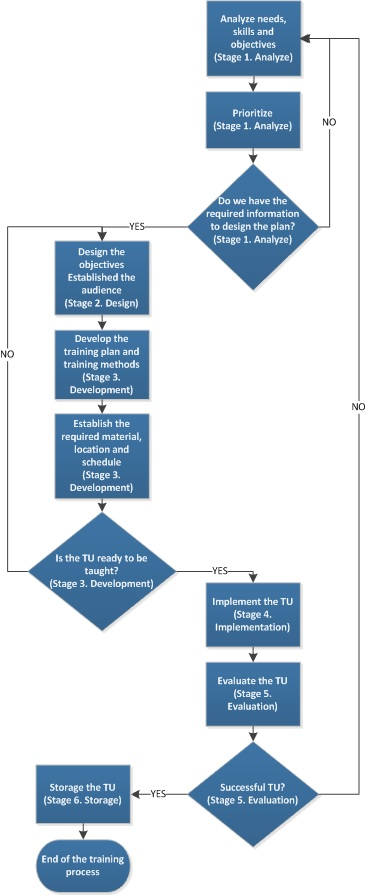
\includegraphics{./figures/Training_process.JPG}
\caption{Training Process flow}
\end{figure}


\subsubsection{Stage One: Analyze}

\begin{itemize}
\item The analyze stage clarifies the instructional problem, establishes the instructional goals and objectives and identifies the learners' existing knowledge and skills. The most important skills to consider should be: 
\begin{itemize}
\item Attitudes
\item Current skills
\item Skill training gap
\item Skill relevancy to tasks
\end{itemize}
With these skills will be established:
\begin{itemize}
\item Project mission
\item Project strategy
\item Core competency needs
\end{itemize}
\item During the analyze stage the Product Owner will carry out:
\begin{itemize}
\item Analysis of needs and skills: knowledge and skills required to undertake each work. The information collected is used to provide an overarching view of the necessary skills and knowledge needed for to effectively carry out the assigned tasks. In order to help with this step the Product owner must fulfill the Training Needs Matrix form {\it{(See Appendice \ref{App:Training-Needs-Matrix})}}.
\item Analysis of the training requirements: Training needs analysis maps the current competencies of the members against the skills and knowledge required for the roles played by them in the project. They are assessed against these requirements and rated on a scale that ranges from “needs development” to “able to train others.”
\item Assessment of viability of training provision to enhance productivity
\item Identification and prioritization of the knowledge, skill gaps and training requirements
\end{itemize}
\item QA manager with the Product Owner, will ensure that qualifications are coherent with the responsibilities defined for the stakeholder’s role as needed for openETCS conformance and for identifying training needs. Qualifications should specify level and type of education, amount and type of experience, previous training, and special skills
\end{itemize}

\subsubsection{Stage Two: Design}

\begin{itemize}
\item In the designing stage the Product Owner defines learning objectives, assessment instruments, and knowledge units. During this stage the Product Owner should: 
\begin{itemize}
\item Design the objectives for developing a quality curricula
\item Select the Trainers. They could be either from different domains within OpenETCS project keeping in view their level of competency in the field of training or also external trainers can be called in the OpenETCS project keeping in view their market reputation and cost of training
\item Define the previous required skills and qualifications to attend the courses. This step will be carried out with the help of the Trainer
\item Establish the audience of the courses
\item Create the Training Methods: define the way that the TU will be taught. This will be carried out with the collaboration of the Trainer.
\item Develop an evaluation plan: method used to test and content inside the training units are evaluated in order to control the effectiveness, stakeholder progress and performance, apply feedback to modify or enhance the TU. With this information the QA Manager and Product Owner will create an evaluation report in which the whole formation process will be evaluated considering each developed register.
\item Create a satisfaction survey form in order to have the opinion of the Stakeholders about the received TU. {\it {(See Appendice \ref{App:Satisfaction-Survey-form})}}
\item Create the training plan.
\end{itemize}
\item During this stage the Trainer, with the supervision of the Product Owner, should:
\begin{itemize}
\item Develop the Training Techniques
\item Do recommendations to solving issues and constraints
\item Establish the minimum required task to do to achieve the objective of the TU successfully.
\end{itemize}
\item QA manager with the Product Owner will ensure that the design have been adequately carried out following each of the steps defined in the training process and having a design that fulfill stakeholders educational needs.
\end{itemize}

\subsubsection{Stage Three: Development}

\begin{itemize}
\item During the development stage the content will be created and assembled by the Trainer, following the guidelines stipulated in the Design stage.
\item Training Units are completed and shall be reviewed by the Product Owner
\begin{itemize}
\item Training Units material, demos and resources will be available.
\end{itemize}
\item Training Units schedule and location will be confirmed. To do these steps the Trainer, Product Owner and Stakeholders will be in contact.
\begin{itemize}
\item Doodle tool will be used with this purpose.
\end{itemize}
\item Training plan will be updated and completed with all the acquired information in order to close it.
\item Product Owner will develop the evaluation system with the collaboration of the QA Manager.
\item Finally, QA manager with the Product Owner will ensure that the development phase fulfill every designing criteria. 
\end{itemize}

\subsubsection{Stage Four: Implementation}
\begin{itemize}
\item During this phase the Stakeholders for the TUs will be contacted by the Product Owner to give them the schedule and agenda. Afterwards the training units will be taught in the schedule and location established and with the available material described in the development stage.
\item The Trainer will maintain the Attendance Record of each Stakeholder. {\it {(See Appendice \ref{App:Attendance-Record})}}
\item The Product Owner will maintain Training Records for each stakeholder. The training records will include information on the following: stakeholder’s name; Job title; Job description, Title of training unit, and Date employee completed the training. {\it {(See Appendice \ref{App:Training-Record})}} that contains the Training Record Form. 
\end{itemize}

\subsubsection{Stage Five: Evaluation}
\begin{itemize}
\item During this stage will be evaluated the TU according to the evaluation plan included in the training plan
\item The Product Owner will send the Stakeholders the satisfaction survey. With the obtained evaluation of the Stakeholders the Product Owner will evaluate the survey results.
\begin{itemize}
\item If the Trainer is from different domains within OpenETCS project the Trainer will review the results of the satisfaction survey and up to date it.
\item For external Trainers the satisfaction survey is sent to them in order to up to date the TU the next time that the TU is taught.  
\end{itemize}
\item The Trainer will send the Product Owner feedback information about Stakeholders, this information is introduced in a Trainer Feedback Report as well as the results from each Stakeholders of the TU. {\it {(See Appendice \ref{App:Trainer-Feedback-Report})}}. With this information the Product Owner will evaluate the fulfillment of the objectives of the training process and will create the Training Evaluation report. {\it {(See Appendice \ref{App:Training-Evaluation-Report})}}
\item Finally, QA Manager review that every register has been fulfilled satisfactorily and the content of each of them is analyzed:
\begin{itemize}
\item Training Needs Matrix
\item Training Records
\item Attendance Record
\item Trainer Feedback Report
\item Satisfaction Surveys
\item Training Storage Records
\item Evaluation report
\end{itemize}
With all the information the Training Evaluation report will be completed if it is needed. This may contain any weakness remained in any Stakeholder by the respective QA manager
\item Futhermore, QA manager will periodically review records of competency training to ensure that all the stakeholders who need specialized training have received the required training. In the case that a Stakeholder has not received or completed the required training, communicating the non-conformance to the Product Owner. 
\end{itemize}

\subsubsection{Stage Six: Storage}
\begin{itemize}
\item During this final stage the Product owner will maintain and save a register containing the training unit material. This material will be categorized, and it will include information like Title of training unit, contact person, recommendations among others. {\it {(See Appendice \ref{App:Training-Storage-Report})}} that contains the form to be fulfilled to correctly identify the saved material.
\item QA Manager has to review that the Storage Register is fulfill correctly with all the created training units and every form has been fill completely and correctly
\end{itemize}

\newpage
\begin{appendices}
   \addappheadtotoc
   \appendixpage
\section{Training Needs Matrix} 
\label{App:Training-Needs-Matrix}
This template has been created as an aid in documenting training needs and delivery mechanisms. This template should be fulfilled by the Product Owner and reviewed by the QA Manager during the first stage of Training planning. 

The content of the template is an example that will vary depending on the type of training, type of Stakeholders, frequency and so on. The Product Owner should have a clear idea of how its product formation should be taught to the different types of Stakeholders.

The template is available in the \href{https://github.com/openETCS/governance/tree/master/Templates}{[governance]} repository

\section{Satisfaction Survey Form} 
\label{App:Satisfaction-Survey-form}
This template has been designed in order to obtain the minimum required information about the quality of the training given to the Stakeholders. This template should be fulfilled by the Stakeholders and reviewed by the Product Owner and QA Manager during the evaluation stage. 

The template is available in the \href{https://github.com/openETCS/governance/tree/master/Templates}{[governance]} repository

\section{Attendance Record} 
\label{App:Attendance-Record}
This template has been created in order to have a control of the attendance of the Stakeholders to each Training Unit. This template should be fulfilled by the Trainer and  reviewed by the Product Owner during the evaluation stage. 

The content of the template is an example. 

The template is available in the \href{https://github.com/openETCS/governance/tree/master/Templates}{[governance]} repository


\section{Training Record} 
\label{App:Training-Record}
This template has been designed to maintain a record of every formation received by each Stakeholder. This template should be fulfilled by the Product Owner and reviewed by the QA Manager during the evaluation stage. 

The content of the template is an example that will vary depending on the Stakeholder, TU and the date the TU is completed. With this template the Product Owner will have a  clear idea of the training receive by each Stakeholder.

The template is available in the \href{https://github.com/openETCS/governance/tree/master/Templates}{[governance]} repository


\section{Trainer Feedback Report} 
\label{App:Trainer-Feedback-Report}
This template has been created as a way of receive the feedback of the Trainer about the Training Unit that he/she has taught. This template should be fulfilled by the Trainer and reviewed by the Product Owner and QA Manager during the evaluation stage. 

This template has an example included; this example will vary depending on the training unit, trainer, stakeholders and so on. With this template and the Stakeholders survey the Product Owner and QA Manager will have a clear idea of how useful the training has been for the Stakeholders and what are the weak and strong points of the training.

The template is available in the \href{https://github.com/openETCS/governance/tree/master/Templates}{[governance]} repository


\section{Training Evaluation Report} 
\label{App:Training-Evaluation-Report}
This template has been designed as a register of the TU evaluation. This template should be fulfilled by the Product Owner and reviewed by the QA Manager during the evaluation stage. 

This template will content description of the complete evaluation of the Training Unit. The most important point of this template is verified that the objectives of the training process have been fulfilled satisfactorily. The weaknesses and strengths of the training unit are highlighted thanks to this template.

The template is available in the \href{https://github.com/openETCS/governance/tree/master/Templates}{[governance]} repository


\section{Training Storage Report} 
\label{App:Training-Storage-Report}
This template has been created as an aid in maintaining a register of the documentation about the Training Units. This template should be fulfilled by the Product Owner and reviewed by the QA Manager during the last stage of Training planning. 

The content of the template is an example that will vary depending on the training, list of content, length of the TU and so on. Thanks to this Storage Record the Product Owner and QA Manager will have a record of every training unit created with its content a small description and recomendations of the Training Unit as well as the training unit length.

The template is available in the \href{https://github.com/openETCS/governance/tree/master/Templates}{[governance]} repository

\end{appendices}
\end{document}
